\section{Overview and Implementation Plan}
This section explains how the Students\&Companies (S\&C) platform will be built, integrated, and tested. The development will happen in phases to ensure that each part of the system is created and tested individually before being connected to the rest. This way, problems can be caught early, and we can avoid larger issues later on.

The implementation will use a combination of two approaches:
\begin{itemize}
    \item  \textbf{Bottom-up} – We’ll start by developing and testing the essential features of the systems that do not require other functionalities to work.
    \item \textbf{Thread-based} – Once the core features are in place, we’ll add new features in parallel. This keeps development moving quickly and gives stakeholders something tangible to see along the way.
\end{itemize}

By using this hybrid method, different teams can work on separate features at the same time, integrating them as soon as they are ready. This not only speeds up development but also reduces the risk of big issues when the full system comes together.

Continuous feedback from stakeholders will be crucial throughout development.

\textbf{Alpha Testing} will be conducted internally by developers and select testers to identify major bugs early in the process. \textbf{Beta Testing} will involve releasing the platform to a limited audience to gather real-world feedback before full deployment.

During the testing phases, logs and reports will be collected to track issues, prioritize fixes, and improve overall system stability. This iterative approach ensures that the platform evolves based on real user interactions, allowing the team to fine-tune the system progressively.

\section{Features Identification}
The system's core features are extracted from the functional and non-functional requirements outlined in the RASD document. These features define how users will interact with the system and how different components will work together to provide a seamless experience. Below is a breakdown of the main features that will be developed, integrated, and tested to ensure the platform meets user expectations and operates smoothly.

\paragraph{[F1] User Authentication (Sign-up, Login, Logout).} This is one of the fundamental features of the platform. It allows users to create an account, log in, and log out securely. Authentication is essential for accessing any part of the system, ensuring that users' data is protected and only authorized individuals can perform specific actions. The platform will support multiple user roles, including students, companies, and university staff, each with different levels of access and privileges. Testing this feature will focus not only on the correctness of login and registration flows but also on ensuring that users are assigned the appropriate role and that permissions are strictly enforced.

\paragraph{[F2] Profile Management.} The profile management feature allows users to build and maintain detailed profiles, which serve as their digital resumes on the platform. Students can input information about their education, skills, and experiences, while companies can create organizational profiles showcasing their internship programs and job opportunities. Profile data is critical for the recommendation system, as it helps match students to internships that align with their qualifications and interests. Companies will also need access to student profiles to evaluate potential candidates during the recruitment process. Testing this feature will focus on ensuring that users can easily create and update their profiles, with real-time validation to prevent errors.

\paragraph{[F3] Internship Management.} This feature allows companies to create, edit, and delete internship listings. Students can search for opportunities based on various filters (location, required skills, etc.) and apply directly through the platform. When an internship is created or updated, the system will automatically notify relevant students who match the internship criteria. This ensures that companies can quickly find suitable candidates and that students do not miss out on potential opportunities. Testing will ensure that internships are properly stored in the database, updates are reflected in real-time, and notifications are sent without delays.

\paragraph{[F4] Recommendation System.} The recommendation system is designed to automate the matching process between students and internships. Using specialized algorithms, the system analyzes student profiles, resumes, and preferences to suggest relevant internship opportunities. This feature reduces the manual effort required from both students and companies, improving the efficiency and accuracy of the recruitment process. The recommendation engine will continuously learn from user interactions and feedback, refining its suggestions over time. Testing this feature will involve simulating different user scenarios to verify that the recommendations are accurate and relevant. Additionally, stress testing will be conducted to ensure the recommendation engine performs well under heavy loads.

\paragraph{[F5] Interview and Task Management.} This feature allows companies to create tasks, assign them to candidates, and evaluate their performance as part of the interview and selection process. Tasks can range from coding challenges to written assignments, providing companies with deeper insights into candidates' abilities. Students receive notifications when tasks are assigned and can submit their work directly through the platform. Companies can then review submissions, score them, and make final selections based on performance. Testing will ensure that tasks are correctly assigned, deadlines are enforced, and submissions are stored securely. The system will also be tested for scalability, as companies may assign tasks to multiple candidates simultaneously.

\paragraph{[F6] Feedback and Complaints.} After internships are completed, students and companies can provide feedback on their experiences. This feedback loop helps improve the matching process by refining the recommendation algorithm and providing valuable insights to users. Additionally, the platform allows users to file complaints if issues arise during an internship. Complaints are forwarded to university staff, who can mediate and work towards resolving disputes. Testing this feature will involve validating the feedback forms, ensuring data integrity, and verifying that complaints are routed to the appropriate parties without delays.

\paragraph{[F7] Notification System.}  The notification system keeps users informed about important events, such as new internship postings, application updates, interview invitations, and complaint resolutions. Notifications will appear within the platform and can also be sent via email for critical actions. This feature ensures that users remain engaged and do not miss essential updates. Testing will focus on the timeliness and accuracy of notifications, ensuring that they trigger correctly based on user actions and system events.

\newpage
\section{Integration Strategy}
The integration of components and the testing of the system should start as soon as the DBMS and the host server are ready. The connections with the Mailing System, GitHub and the External Tools are not required since the starting moment, but will be necessary once the corresponding features will be integrated. As explained before the integration will follow a bottom-up approach.
\\
Starting from the model, which will be tested alongside a proper driver, 


\begin{figure}[H]
    \begin{center}
        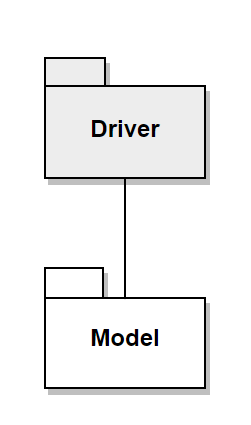
\includegraphics[width=0.2\linewidth]{Integration/I1.png}
        \label{fig:Integration_1}%
    \end{center}
\end{figure}


The integration of components will proceed with the Login and Registration features:

\begin{figure}[H]
    \begin{center}
        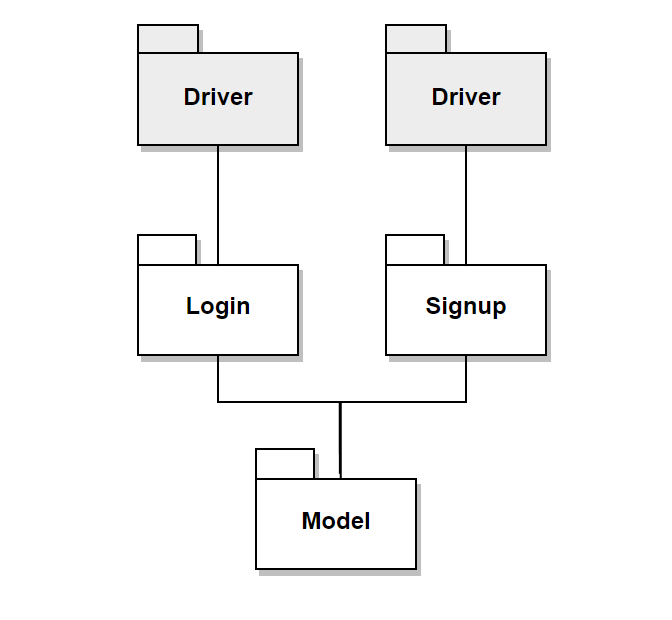
\includegraphics[width=0.4\linewidth]{Integration/I2.png}
        \label{fig:Integration_2}%
    \end{center}
\end{figure}

Once they will be developed and tested, it will be the turn of the components that perform a creation feature and their drivers:

\begin{figure}[H]
    \begin{center}
        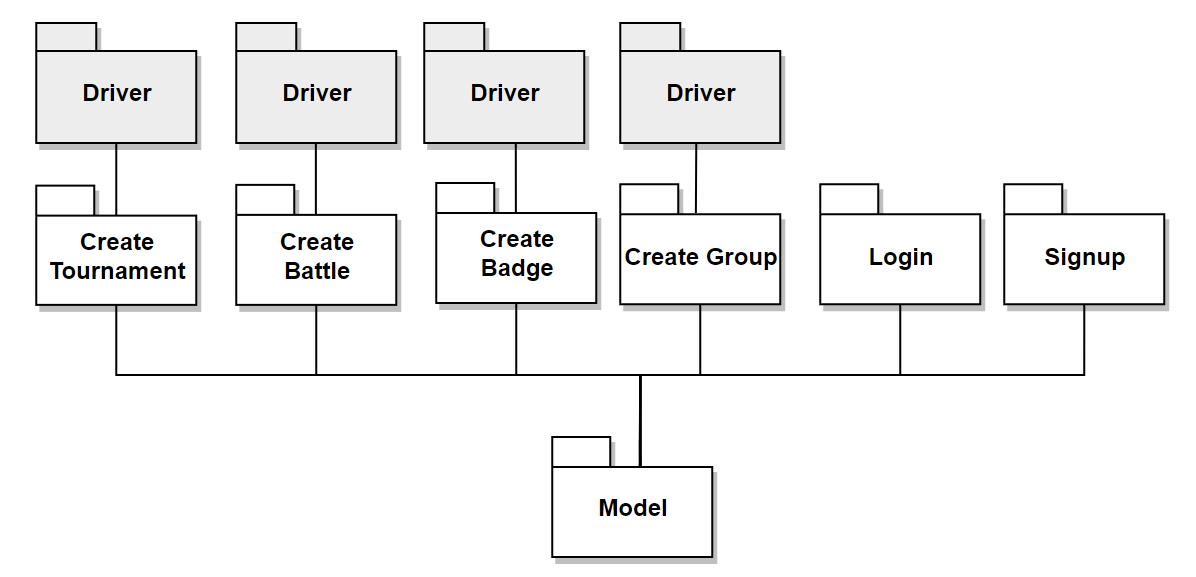
\includegraphics[width=0.8\linewidth]{Integration/I3.png}
        \label{fig:Integration_3}%
    \end{center}
\end{figure}

Now it is possible to create Tournaments, Battles, Groups and Badges functions to view those elements’ pages or the search components can be integrated.


\begin{figure}[H]
    \begin{center}
        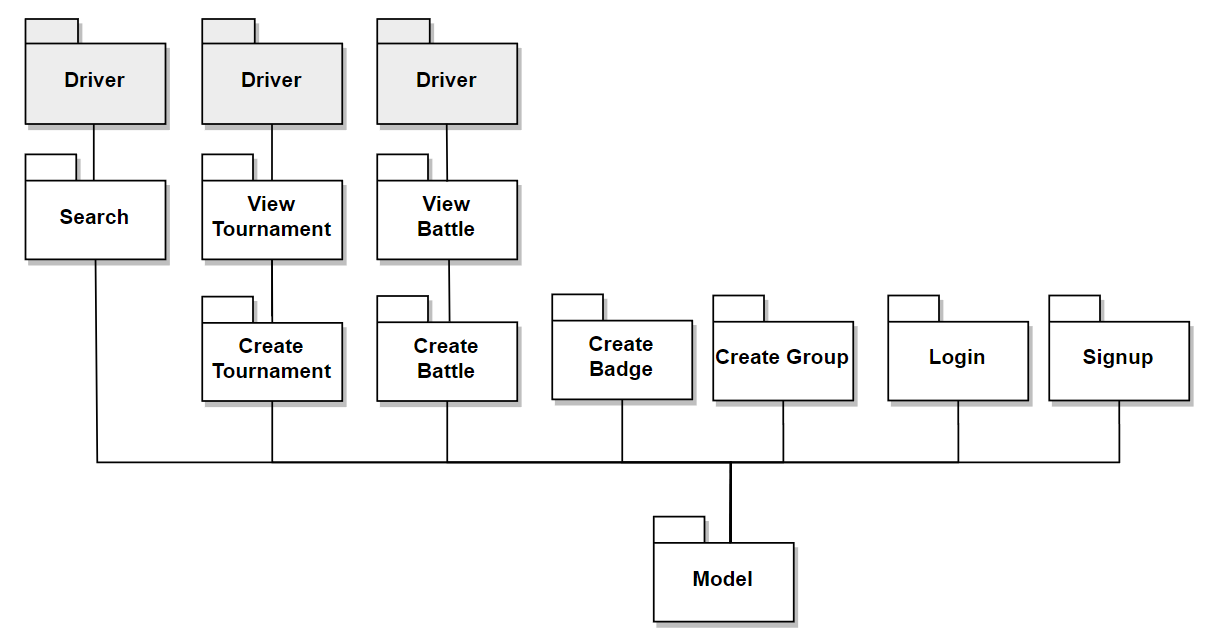
\includegraphics[width=0.8\linewidth]{Integration/I4.png}
        \label{fig:Integration_4}%
    \end{center}
\end{figure}

The last missing components in the context of Tournaments and Battles are the Join features, which will be integrated in parallel with the possibility to open Users’ profiles and to modify Badges parameters for the EDs.


\begin{figure}[H]
    \begin{center}
        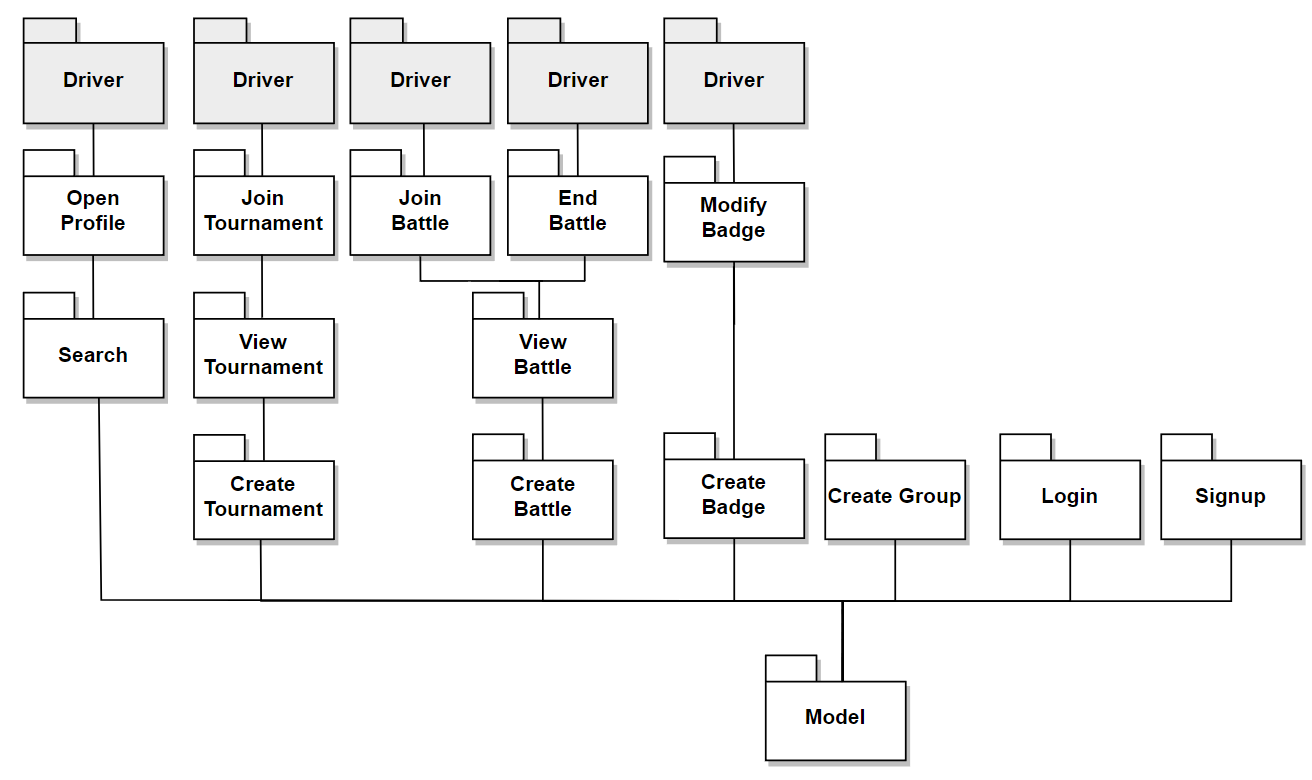
\includegraphics[width=0.8\linewidth]{Integration/I5.png}
        \label{fig:Integration_5}%
    \end{center}
\end{figure}

For the sake of simplicity, the previously integrated components are represented grouped in their Manager component (let the ‘Tournament Manager’ contain every Tournament-related component, and so on). Evaluation features will come next.

\begin{figure}[H]
    \begin{center}
        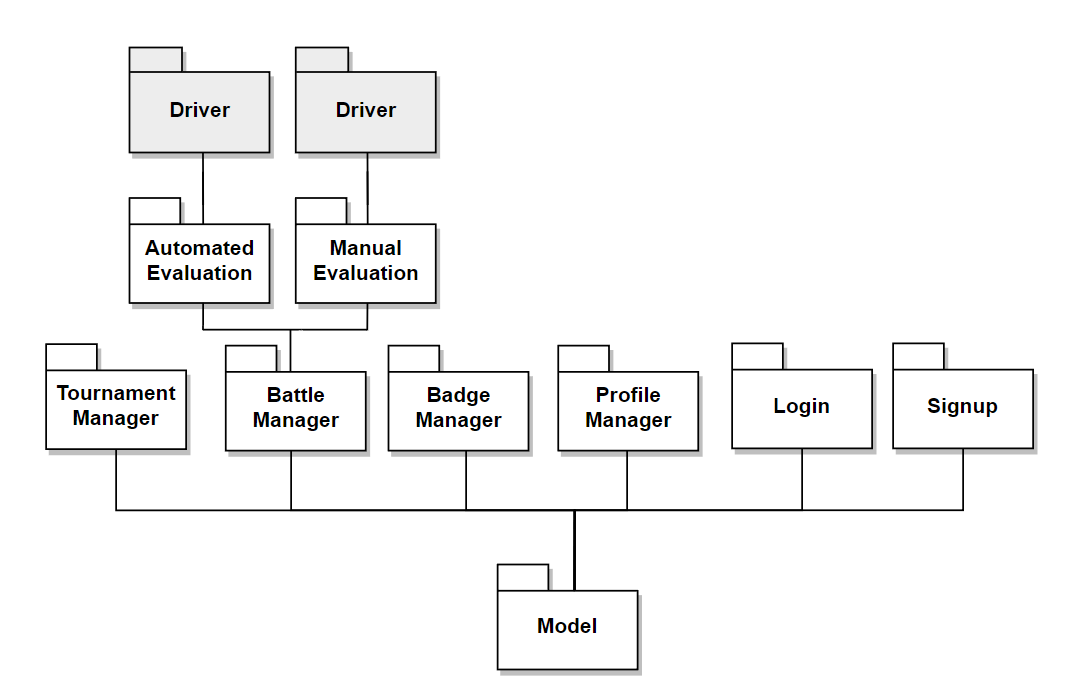
\includegraphics[width=0.8\linewidth]{Integration/I6.png}
        \label{fig:Integration_6}%
    \end{center}
\end{figure}

Once the Evaluation features are integrated, they will be considered as the same in the ‘Evaluation Manager’. Then Notification Manager will be the next to be integrated and tested.


\begin{figure}[H]
    \begin{center}
        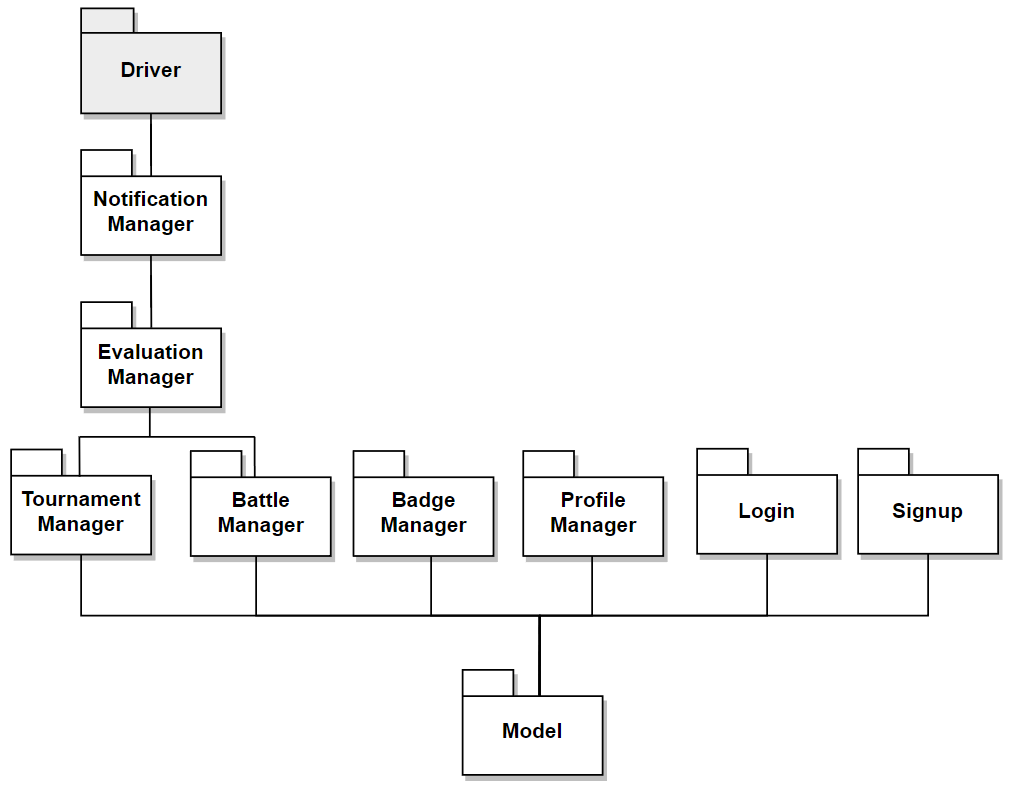
\includegraphics[width=0.8\linewidth]{Integration/I7.png}
        \label{fig:Integration_7}%
    \end{center}
\end{figure}

The last component that has to be integrated is the dashboard Manager, that is essential for the correct workflow of the user interface.


\begin{figure}[H]
    \begin{center}
        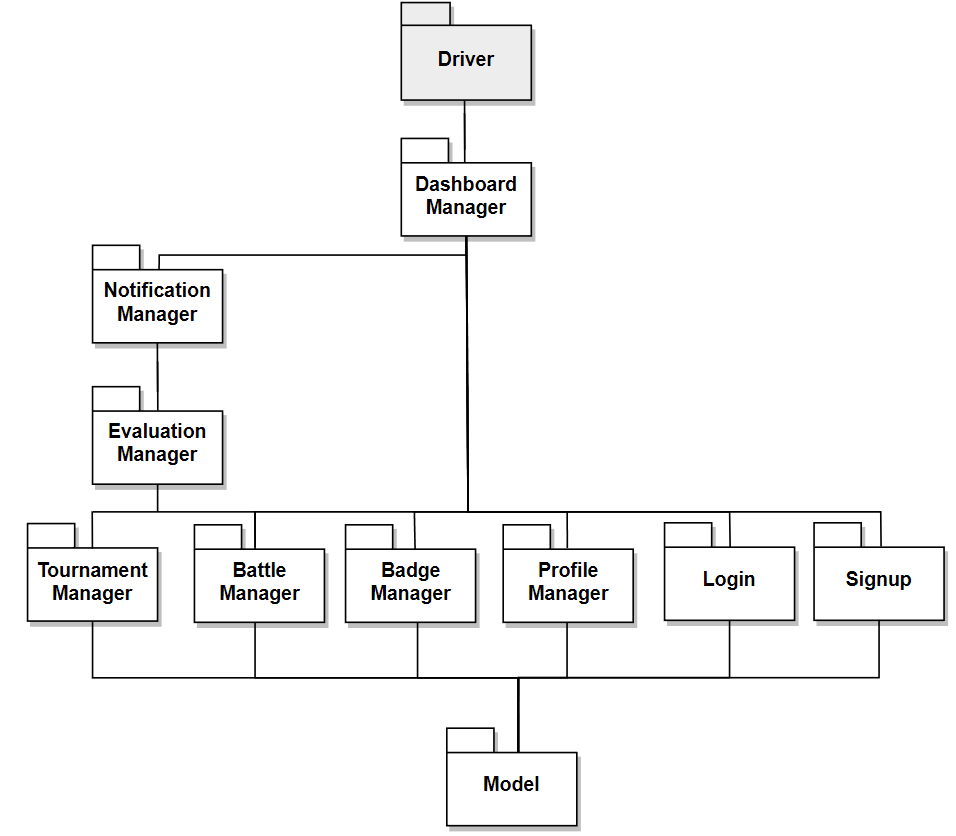
\includegraphics[width=0.8\linewidth]{Integration/I8.png}
        \label{fig:Integration_8}%
    \end{center}
\end{figure}

After the removal of the Dashboard Manager’s Driver, the final system is as follows.

\begin{figure}[H]
    \begin{center}
        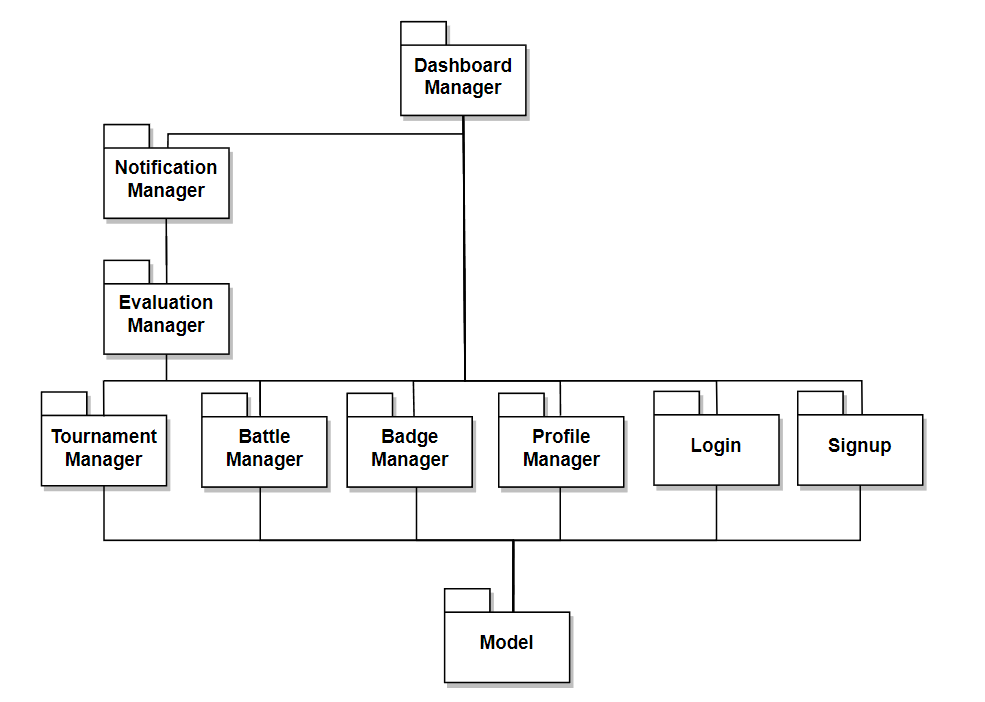
\includegraphics[width=0.8\linewidth]{Integration/IFinal.png}
        \label{fig:Integration_final}%
    \end{center}
\end{figure}



\section{System Testing Strategy}

It is necessary to check that each newly developed component works properly before integrating it with the system by the use of Drivers. Once a new component is integrated to the system, it must be checked with a new Driver that the new component is properly integrated, that the modules’ properties still hold and that the integrated system follows the correct workflow. 
Once every component is integrated, it will be needed to test the system as a whole to ensure the proper workflow is followed and the absence of bugs. In order to do so the following kinds of testing will be applied. 

\begin{itemize}
    \item \textbf{Functional Testing: }Functional Testing will be performed on the system to guarantee that the workflow is correct and consistent with the functionalities described in the RASD document, checking the fulfillment of goals, requirements and use cases and the possibility to correctly simulate the described scenarios. 
    \item \textbf{Load Testing:} Load Testing is useful in order to find eventual memory leaks, buffer overflows and bad management of memory.
    \item \textbf{Performance Testing:} The system will undergo this kind of testing in order to identify bottlenecks and to observe the resilience of the system under heavy workload, keeping in mind that the system shall support many users working simultaneously keeping response times as low as possible, following what is stated in the \textit{RASD document, section 3.3}. This will also help to identify optimization possibilities in the software’s algorithms.
    \item \textbf{Stress Testing:} In order to make sure that the system is capable of recovering itself after a failure, Stress Testing will be adopted, by simulating lots of concurrent users or reducing the system’s computational resources.
    \item \textbf{User Interface Testing:} It is important that the system correctly works on different kinds of devices, and different browsers as stated during the Requirements Analysis, testing the usability and accessibility of the web app on every possible platform, for both kinds of users: EDs and STs. 
\end{itemize}